% The light cone of an event A, one dimension of space suppressed: future and
% past cones, the region elsewhere, a worldline through A, and two events.
\documentclass[tikz,border=1pt]{standalone}
% Shared preamble for the standalone figures: the book's fonts, palette and
% drawing styles. Figures are drawn at their final printed size. A column is
% 3.35in (241pt) wide; a figure across both columns is 7in (505pt) wide.

\usepackage[T1]{fontenc}
\usepackage{newpxtext}
\usepackage[varbb]{newpxmath}
\usepackage[semibold,scale=0.95,lining]{sourcesanspro}
\usepackage{xcolor}
% Palette shared by the book and by the standalone figures in figures/src.
% One main hue (blue), one accent (orange), and a few roles used sparingly.

\definecolor{seblue}{HTML}{1D5B8F}    % headings, worked examples, main curves
\definecolor{seblueDark}{HTML}{123E63}
\definecolor{seorange}{HTML}{DC7A26}  % thought experiments, light and light cones
\definecolor{seteal}{HTML}{1F8577}    % checks, travellers and ships
\definecolor{sered}{HTML}{C0392B}     % negative energy, tension, violations
\definecolor{seviolet}{HTML}{5E548E}  % going deeper
\definecolor{sesand}{HTML}{8C6A3F}    % history
\definecolor{segray}{HTML}{6B7480}    % axes, guides, secondary labels
\definecolor{selight}{HTML}{D5DAE1}   % grids and faint rules

\usepackage{siunitx}
\usepackage{fontawesome5}
\usepackage{tikz}
\usetikzlibrary{arrows.meta,calc,positioning,decorations.pathreplacing,
  decorations.markings,shapes.geometric,fadings,shadings,patterns,3d,
  intersections,backgrounds}
\usepackage{pgfplots}
\pgfplotsset{compat=1.18}
\usepgfplotslibrary{fillbetween,groupplots,colormaps}

\tikzset{
  >={Latex[length=2.1mm,width=1.4mm]},
  every picture/.style={line cap=round, line join=round},
  lbl/.style={font=\sffamily\footnotesize, text=black!85},
  smalllbl/.style={font=\sffamily\scriptsize, text=black!75},
  guide/.style={segray, line width=0.4pt},
  axisline/.style={segray, line width=0.5pt, -{Latex[length=1.7mm,width=1.1mm]}},
  light/.style={seorange, line width=0.9pt},
  lightdash/.style={seorange, line width=0.9pt, dash pattern=on 3pt off 2pt},
  ship/.style={seteal, line width=1.4pt},
  cone/.style={fill=seorange!22, draw=seorange!85!black, line width=0.35pt},
}

\pgfplotsset{
  se axis/.style={
    axis lines=left,
    axis line style={segray, line width=0.5pt, -{Latex[length=1.6mm,width=1.1mm]}},
    tick style={segray, line width=0.4pt},
    major tick length=2.5pt,
    tick label style={font=\sffamily\scriptsize, text=black!75},
    label style={font=\sffamily\footnotesize, text=black!85},
    every axis plot/.append style={line width=1.1pt},
    legend style={font=\sffamily\scriptsize, draw=none, fill=none},
    scaled ticks=false,
    xticklabel={\sansnum{\tick}}, yticklabel={\sansnum{\tick}},
  },
}

% Numbers in figures are set in the sans-serif text font, with a true minus.
\sisetup{mode=text, reset-text-family=false, reset-text-series=false,
  reset-text-shape=false, drop-zero-decimal, group-minimum-digits=5}
% Tick values arrive as long decimals (1.5000000000); parse them first.
\newcommand{\sansnum}[1]{\begingroup\pgfkeys{/pgf/fpu=false}%
  \pgfmathparse{1*(#1)}\num{\pgfmathresult}\endgroup}

\begin{document}
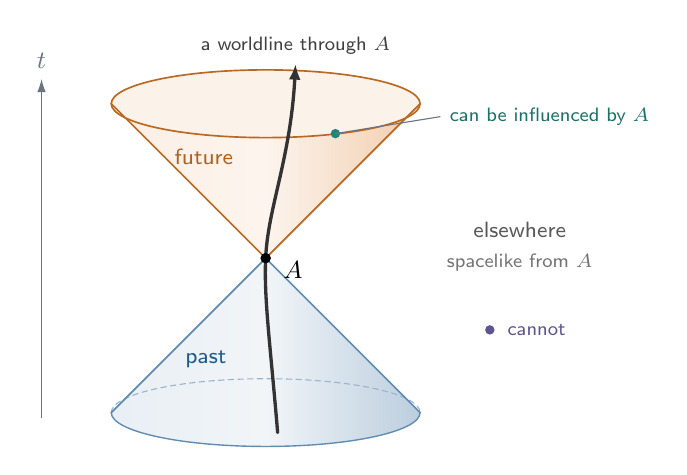
\begin{tikzpicture}[x=36pt, y=36pt]
\def\R{1.55}\def\e{0.34}
% past cone (drawn first)
\shade[left color=seblue!10, right color=seblue!30, middle color=seblue!6]
  (0,0) -- (-\R,-\R) arc[start angle=180, end angle=360, x radius=\R, y radius=\e] -- cycle;
\draw[seblue!70, line width=0.5pt] (-\R,-\R) arc[start angle=180, end angle=360, x radius=\R, y radius=\e];
\draw[seblue!45, line width=0.4pt, dash pattern=on 2pt off 1.5pt] (-\R,-\R) arc[start angle=180, end angle=0, x radius=\R, y radius=\e];
\draw[seblue!70, line width=0.6pt] (0,0) -- (-\R,-\R) (0,0) -- (\R,-\R);
% worldline, lower half
\draw[black!80, line width=1.2pt] (0.12,-1.75) .. controls (0.05,-0.9) and (-0.02,-0.4) .. (0,0);
% future cone
\shade[left color=seorange!12, right color=seorange!38, middle color=seorange!8]
  (0,0) -- (-\R,\R) arc[start angle=180, end angle=360, x radius=\R, y radius=\e] -- cycle;
\fill[seorange!10] (0,\R) ellipse[x radius=\R, y radius=\e];
\draw[seorange!85!black, line width=0.6pt] (0,\R) ellipse[x radius=\R, y radius=\e];
\draw[seorange!85!black, line width=0.6pt] (0,0) -- (-\R,\R) (0,0) -- (\R,\R);
% worldline, upper half
\draw[black!80, line width=1.2pt, -{Latex[length=2mm,width=1.5mm]}] (0,0) .. controls (0.02,0.5) and (0.25,1.0) .. (0.3,1.95);
\node[smalllbl, anchor=south] at (0.3,1.95) {a worldline through $A$};
% axis
\draw[axisline] (-2.25,-1.6) -- (-2.25,1.8) node[anchor=south, font=\small] {$t$};
% event A and labels
\fill (0,0) circle (1.9pt);
\node[font=\small, anchor=west] at (0.08,-0.12) {$A$};
\node[lbl, text=seorange!80!black] at (-0.62,1.02) {future};
\node[lbl, text=seblue] at (-0.6,-1.02) {past};
\node[lbl, text=black!65, align=center] at (2.55,0.28) {elsewhere};
\node[smalllbl, text=black!55, align=center] at (2.55,-0.05) {spacelike from $A$};
% two events
\fill[seteal] (0.7,1.25) circle (1.7pt);
\draw[guide] (0.7,1.25) -- (1.75,1.42) node[smalllbl, anchor=west, text=seteal!85!black] {can be influenced by $A$};
\fill[seviolet] (2.25,-0.72) circle (1.7pt);
\node[smalllbl, anchor=west, text=seviolet] at (2.33,-0.72) {cannot};
\end{tikzpicture}
\end{document}
